\chapter{Групповая скорость, фермионное исключение и море Дирака}

\section{Фазовая скорость и групповая скорость}

\begin{classroomqa}
\lecturetimestamp{00:00:07}
\audiencequestion{Что такое групповая скорость и фазовая скорость?}
\lecturerresponse{Фазовая скорость отслеживает точку фиксированной фазы в плоской волне. Обычно она не описывает движение измеримого объекта. Групповая скорость отслеживает огибающую волнового пакета и является скоростью, связанной с частицами, сигналами и потоком вероятности.}
\end{classroomqa}

Начнём с плоской волны,
\begin{equation}
\psi(x,t)=e^{i(kx-\omega t)},
\end{equation}
или с её вещественной формы,
\begin{equation}
\psi(x,t)=\sin(kx-\omega t).
\end{equation}
Гребень, впадина или любая другая точка с фиксированной фазой движется так, что
\begin{equation}
kx-\omega t=\text{constant}.
\end{equation}
Если для удобства выбрать константу равной нулю, получим
\begin{equation}
x=\frac{\omega}{k}t,
\qquad
v_{\mathrm{phase}}=\frac{\omega}{k}.
\end{equation}
Поскольку \(\omega=2\pi/T\) и \(k=2\pi/\lambda\),
\begin{equation}
v_{\mathrm{phase}}=\frac{\omega}{k}=\frac{\lambda}{T}.
\end{equation}
Это просто расстояние, на которое данная фаза продвигается за один период.

Для нерелятивистской волны Schr\"odinger, при \(\hbar=1\) энергия и импульс равны \(\omega\) и \(k\), так что
\begin{equation}
\omega(k)=\frac{k^2}{2m}.
\end{equation}
Следовательно, её фазовая скорость равна
\begin{equation}
v_{\mathrm{phase}}=\frac{k}{2m}.
\end{equation}
Однако обычная скорость частицы с импульсом \(k\) равна \(k/m\). Несовпадение на множитель 2 — первое предупреждение о том, что движение фазы плоской волны не есть движение частицы.

Есть и ещё более резкое предупреждение. Прибавим одну и ту же константу \(C\) ко всем частотам:
\begin{equation}
\omega(k)\longrightarrow \omega(k)+C.
\end{equation}
Эта константа может, например, представлять общий вклад энергии покоя, такой как \(mc_{\mathrm{light}}^2\), но её конкретное название несущественно. Здесь \(C\) — это сдвиг энергии, а не скорость света. Тогда фазовая скорость становится
\begin{equation}
v_{\mathrm{phase}}\longrightarrow
\frac{\omega(k)+C}{k}
=v_{\mathrm{phase}}+\frac{C}{k}.
\end{equation}
Однако добавление одной и той же константы к каждой энергии не изменяет ни одной разности энергий и, следовательно, не изменяет никакой нерелятивистской физики.

Это можно увидеть непосредственно из волновой функции. Запишем общее поле Schr\"odinger как сумму или интеграл по модам,
\begin{equation}
\psi(x,t)=\sum_k a_k e^{ikx}e^{-i\omega(k)t},
\end{equation}
опуская множители нормировки. После сдвига
\begin{align}
\psi(x,t)
&\longrightarrow
\sum_k a_k e^{ikx}e^{-i[\omega(k)+C]t}
\\
&=e^{-iCt}\psi(x,t).
\end{align}
Каждая мода приобрела одну и ту же зависящую от времени фазу. Сопряжённое поле приобретает противоположную фазу, и поэтому
\begin{equation}
\begin{aligned}
\psi^*(x,t)\psi(x,t)
&\longrightarrow
e^{iCt}e^{-iCt}\psi^*(x,t)\psi(x,t)
\\
&=\psi^*(x,t)\psi(x,t).
\end{aligned}
\end{equation}
То же сокращение происходит и в средних значениях. Величина, которая меняется при сдвиге нуля энергии, не может быть физической скоростью распространения частицы Schr\"odinger. Следовательно, фазовая скорость отчасти условна.

Локализованная частица представляется не одной бесконечной плоской волной, а пакетом. Составляющие волны складываются конструктивно в области пакета и деструктивно вне её. Движение этой картины уже можно найти из двух близких волн:
\begin{equation}
\psi(x,t)=
\sin(kx-\omega t)+
\sin(k'x-\omega't),
\end{equation}
где \(k'\) близко к \(k\) и \(\omega'=\omega(k')\). Геометрическое место конструктивной интерференции задаётся условием совпадения их фаз,
\begin{equation}
kx-\omega t=k'x-\omega't.
\end{equation}
Отсюда
\begin{equation}
(k-k')x=(\omega-\omega')t,
\end{equation}
и усиленная картина движется согласно
\begin{equation}
x=\frac{\omega-\omega'}{k-k'}t.
\end{equation}
Переходя к пределу соседних волн, получаем
\begin{equation}
x=\frac{d\omega}{dk}t,
\qquad
v_{\mathrm{group}}=\frac{d\omega}{dk}.
\end{equation}
Это скорость огибающей---локализованного сгустка, возникающего из-за интерференции составляющих волн.

Для нерелятивистского дисперсионного соотношения, включая произвольный сдвиг,
\begin{equation}
\omega(k)=\frac{k^2}{2m}+C,
\end{equation}
групповая скорость равна
\begin{equation}
v_{\mathrm{group}}
=\frac{d}{dk}\left(\frac{k^2}{2m}+C\right)
=\frac{2k}{2m}
=\frac{k}{m}.
\end{equation}
Аддитивная константа исчезла, и результат в точности совпадает с классической скоростью частицы.

\begin{classroomqa}
\lecturetimestamp{00:16:35}
\audiencequestion{Исчезает ли множитель 2 в групповой скорости?}
\lecturerresponse{Да. При дифференцировании \(k^2\) получается \(2k\), что сокращает двойку в \(2m\). В результате выходит \(k/m\).}
\end{classroomqa}

Следовательно, групповая скорость — это скорость, наиболее тесно связанная с классическим движением частицы. Она также является скоростью, существенной для распространения пакета и, в обычных рассматриваемых здесь обстоятельствах, для распространения сигналов. Фазовая скорость не обязана иметь ни того, ни другого смысла.

\subsection{Безмассовые и массивные релятивистские волны}

\begin{classroomqa}
\lecturetimestamp{00:17:47}
\audiencequestion{Имеет ли это отношение к утверждениям, что свет может распространяться быстрее света?}
\lecturerresponse{Нет. Эти утверждения поднимают отдельный вопрос. Родственный расчёт действительно показывает, что фаза может двигаться быстрее света, тогда как физическая групповая скорость остаётся досветовой, но это не описывает сигнал, обгоняющий свет.}
\end{classroomqa}

\begin{classroomqa}
\lecturetimestamp{00:18:05}
\audiencequestion{Имеется ли в виду здесь знакомый пример, в котором фазовая скорость превышает скорость света, тогда как групповая остаётся меньше неё?}
\lecturerresponse{Да. Та же картина возникает для релятивистской волны с ненулевой массой, и она прямо следует из релятивистского соотношения энергия--импульс.}
\end{classroomqa}

Положим \(\hbar=c_{\mathrm{light}}=1\). Релятивистское соотношение имеет вид
\begin{equation}
E=\sqrt{p^2+m^2},
\qquad
\omega(k)=\sqrt{k^2+m^2}.
\end{equation}
Полезно сначала установить безмассовый случай. При \(m=0\),
\begin{equation}
\omega=|k|.
\end{equation}
На правой ветви, где \(k>0\), \(\omega=k\), и поэтому
\begin{equation}
v_{\mathrm{phase}}=\frac{\omega}{k}=1,
\qquad
v_{\mathrm{group}}=\frac{d\omega}{dk}=1.
\end{equation}
На левой ветви обе скорости имеют соответствующий отрицательный знак. В любом случае их скорость по модулю равна скорости света. Поскольку дисперсионное соотношение линейно на каждой ветви, все фурье-компоненты на этой ветви движутся с одной и той же скоростью.

Для массивной частицы при \(k>0\),
\begin{equation}
v_{\mathrm{phase}}
=\frac{\omega}{k}
=\sqrt{\frac{k^2+m^2}{k^2}}>1,
\end{equation}
тогда как
\begin{equation}
v_{\mathrm{group}}
=\frac{d\omega}{dk}
=\frac{k}{\sqrt{k^2+m^2}}<1.
\end{equation}
При \(k<0\) обе скорости меняют знак, а их модули подчиняются тем же неравенствам. Таким образом, фаза может двигаться быстрее света, тогда как пакет, частица, энергия и сигнал движутся медленнее света. Для этого конкретного дисперсионного соотношения и при \(k\neq0\),
\begin{equation}
v_{\mathrm{phase}}v_{\mathrm{group}}=1.
\end{equation}
Это обратное соотношение — случайная особенность дисперсионного соотношения с квадратным корнем, а не общее свойство волн.

\begin{figure}
\centering
\includegraphics[width=0.72\textwidth]{lecture_05_figure_03.png}
\caption{Нерелятивистское и релятивистское дисперсионные соотношения, с фазовой скоростью \(\omega/k\) и групповой скоростью \(d\omega/dk\).}
\lectureframe{00:35:52}
\end{figure}

\begin{classroomqa}
\lecturetimestamp{00:23:41}
\audiencequestion{Связана ли дисперсия с тем, что скорость волны зависит от частоты?}
\lecturerresponse{Да. Когда \(\omega(k)\) линейно, каждая фурье-компонента имеет одну и ту же групповую скорость, и пакет может сохранять свою форму. Когда \(\omega(k)\) нелинейно, разные компоненты движутся с разными скоростями, так что пакет диспергирует и меняет форму. Низкочастотный звук приблизительно недисперсионен, когда его частота почти пропорциональна волновому числу.}
\end{classroomqa}

Фазовая скорость обычно не переносит ни сигнал, ни энергию, ни поток вероятности. Её численное значение можно даже изменить, сдвинув нуль энергии. Групповая скорость — это физически значимое движение достаточно узкого пакета.

\begin{classroomqa}
\lecturetimestamp{00:25:14}
\audiencequestion{Можно ли измерить фазовую скорость у фотона?}
\lecturerresponse{В вакууме у фотона линейная дисперсия, поэтому его фазовая и групповая скорости совпадают, и обе равны скорости света. В материальной среде дисперсионное соотношение меняется, и фазовая и групповая скорости не обязаны совпадать.}
\end{classroomqa}

\begin{classroomqa}
\lecturetimestamp{00:25:50}
\audiencequestion{Ограничивается ли это обсуждение волновыми пакетами, которые не расплываются со временем?}
\lecturerresponse{Пакет остаётся нерасплывающимся только тогда, когда все его фурье-компоненты имеют одну и ту же скорость, что соответствует линейному дисперсионному соотношению в соответствующем диапазоне. При нелинейной дисперсии компоненты расходятся, и пакет расплывается.}
\end{classroomqa}

Вопросы о световых конусах и релятивистской причинной структуре требуют большего, чем различение фазовой и групповой скорости, и остаются вне рамок этого расчёта.

\section{Трансляционная симметрия и законы сохранения}

Те же фазы плоских волн дают компактное описание законов сохранения. Начнём с сохранения энергии. Поле уничтожения, действующее на входящую частицу с энергией \(\omega_j\), вносит временной множитель
\begin{equation}
e^{-i\omega_j t},
\end{equation}
тогда как поле рождения, создающее выходящую частицу с энергией \(\omega'_r\), вносит
\begin{equation}
e^{+i\omega'_r t}.
\end{equation}
Для нескольких входящих и выходящих частиц их произведение имеет вид
\begin{equation}
\exp\!\left[
i\left(\sum_r\omega'_r-\sum_j\omega_j\right)t
\right].
\end{equation}
Если взаимодействие может происходить в любой момент времени с одной и той же амплитудой, то амплитуда включает интеграл по времени взаимодействия:
\begin{equation}
\begin{aligned}
&\int_{-\infty}^{\infty}dt\,
\exp\!\left[
i\left(\sum_r\omega'_r-\sum_j\omega_j\right)t
\right]
\\
&\quad =2\pi\,
\delta\!\left(\sum_r\omega'_r-\sum_j\omega_j\right).
\end{aligned}
\end{equation}
Дельта-функция требует, чтобы суммарная энергия выходящих частиц равнялась суммарной энергии входящих. Одинаковая амплитуда в каждый возможный момент взаимодействия — это инвариантность относительно трансляций по времени, и она приводит к сохранению энергии.

Пространственная трансляция приводит к сохранению импульса тем же механизмом. Рассмотрим физический распад одной частицы на две, в котором входящая частица с импульсом \(k\) исчезает, а появляются две частицы с импульсами \(k'_1\) и \(k'_2\). Локальное взаимодействие в положении \(x\) содержит одно поле уничтожения и два поля рождения,
\begin{equation}
\mathcal{O}(x)=\psi^\dagger(x)\psi^\dagger(x)\psi(x).
\end{equation}
Опуская временную зависимость и нормировку, соответствующие модовые множители имеют вид
\begin{align}
\psi(x)&\supset a_k e^{ikx},
\\
\psi^\dagger(x)&\supset a_{k'_1}^\dagger e^{-ik'_1x},
\qquad
\psi^\dagger(x)\supset a_{k'_2}^\dagger e^{-ik'_2x}.
\end{align}
В матричном элементе
\begin{equation}
\langle k'_1,k'_2|\mathcal{O}(x)|k\rangle,
\end{equation}
оператор уничтожения убирает входящую частицу, а два оператора рождения создают исходящие частицы. После выполнения этих операторных действий остается зависящий от положения множитель
\begin{equation}
e^{-ik'_1x}e^{-ik'_2x}e^{ikx}
=e^{i(k-k'_1-k'_2)x}.
\end{equation}
Поскольку никакое положение не является выделенным, интегрируют по всем возможным положениям распада:
\begin{equation}
\int_{-\infty}^{\infty}dx\,
e^{i(k-k'_1-k'_2)x}
=2\pi\delta(k-k'_1-k'_2).
\end{equation}
Следовательно, для оставшейся амплитуды выполняется
\begin{equation}
k=k'_1+k'_2.
\end{equation}
В трех измерениях в том же вычислении используются \(d^3x\), векторы импульса, набранные полужирным, и трехмерная дельта-функция. В этом рассуждении ничто не зависит от того, что имеется только одна входящая частица или две исходящие. При произвольных числах частиц интегрирование по общему положению взаимодействия дает
\begin{equation}
\delta^{(3)}\!\left(
\sum_j\mathbf{k}_j-\sum_r\mathbf{k}'_r
\right).
\end{equation}
Одинаковость амплитуды во всех положениях и есть инвариантность относительно пространственных трансляций, и она приводит к сохранению импульса точно так же, как одинаковость амплитуды во все моменты времени приводит к сохранению энергии.

Третий пример — глобальное фазовое вращение,
\begin{equation}
\psi\longrightarrow e^{i\lambda}\psi,
\qquad
\psi^\dagger\longrightarrow e^{-i\lambda}\psi^\dagger.
\end{equation}
Амплитуда взаимодействия инвариантна, когда фазы, вносимые полями уничтожения и рождения, сокращаются. Для поля, несущего электрический заряд, это равенство заряда, удаляемого из начального состояния и восстанавливаемого в конечном, есть сохранение заряда. Тем самым временные трансляции, пространственные трансляции и глобальные фазовые вращения показывают, как поля, создающие и уничтожающие частицы, кодируют сохранение энергии, импульса и заряда.

\begin{classroomqa}
\lecturetimestamp{00:37:52}
\audiencequestion{Означает ли интегрирование по пространству интегрирование по всем трем пространственным измерениям?}
\lecturerresponse{Да. Три интегрирования дают дельта-функцию для трех компонент импульса, так что сохраняются все три компоненты полного импульса.}
\end{classroomqa}

\begin{classroomqa}
\lecturetimestamp{00:38:03}
\audiencequestion{Определяет ли эта модель относительные вероятности разных способов разделить сохраняющийся импульс?}
\lecturerresponse{Нет. Это простое выражение фиксирует сумму исходящих импульсов, но в остальном никак не выделяет их распределение. Для относительных вероятностей нужна дополнительная динамическая информация.}
\end{classroomqa}

\begin{classroomqa}
\lecturetimestamp{00:39:04}
\audiencequestion{Почему сумма операторов уничтожения сводится к члену, соответствующему занятой импульсной моде?}
\lecturerresponse{Оператор уничтожения, действующий на пустую моду, дает нулевой вектор. Если состояние содержит одну частицу только в моде \(k_0\), то все члены, кроме члена с \(k=k_0\), обращаются в нуль.}
\end{classroomqa}

Например,
\begin{equation}
\sum_k a_k e^{ikx}|1_{k_0}\rangle
=e^{ik_0x}|0\rangle,
\end{equation}
с точностью до нормировки: все операторы уничтожения, соответствующие пустым модам, дают нулевой вектор.

\section{Бозонное усиление и фермионный запрет}

Бозоны допускают любое неотрицательное число заполнения в одночастичном состоянии, и алгебра их операторов рождения действительно благоприятствует уже занятому состоянию. Для одной бозонной моды в нормированном соглашении для числовых состояний усиление заселенности записывается как\footnote{В лекции усиление заселенности формулируется в виде квадратного корня; это уравнение с индексами представляет его стандартную форму для числовых состояний.}
\begin{equation}
a^\dagger|n\rangle=\sqrt{n+1}\,|n+1\rangle.
\end{equation}
Предположим, что возбужденный атом может испустить фотон во множество возможных мод. В отсутствие других фотонов различные направления и импульсы реализуются со своим обычным распределением вероятностей. Если некоторая мода уже содержит много фотонов---все с одинаковыми импульсом, энергией и частотой---то испускание в эту моду усиливается соответствующим корневым фактором заселенности. Атом предпочтительно добавляет свой фотон к уже заселенному состоянию. Это и есть вынужденное излучение, конкретное проявление бозонного скучивания.

Фермионы ведут себя противоположным образом. Два тождественных фермиона не могут занимать одно и то же квантовое состояние. Принцип запрета впервые возник в атомной физике, где два электрона в атоме не могут иметь одинаковые квантовые числа, но он не ограничивается атомами: тождественные фермионы нигде не могут занимать одно и то же полное одночастичное состояние.

Разложение поля сначала выглядит точно так же, как и бозонное. В конечном ящике можно написать
\begin{equation}
\psi(x)=\sum_k A_k e^{ikx},
\qquad
\psi^\dagger(x)=\sum_k A_k^\dagger e^{-ikx}.
\end{equation}
Для непрерывного импульса суммы превращаются в интегралы. Противоположный знак в сопряженной пространственной фазе следует из эрмитова сопряжения. Эта часть построения нерелятивистская; релятивистские фермионы появятся только в конце.

Состояние поля по-прежнему задается числом заполнения для каждой моды, но теперь каждое такое число может быть только нулем или единицей:
\begin{equation}
|n_{k_1},n_{k_2},\ldots\rangle,
\qquad n_k\in\{0,1\}.
\end{equation}
Никаких дополнительных релятивистских типов частиц с, скажем, не более чем тремя частицами на состояние или не менее чем семью частицами на состояние не существует. Установление того, что бозонная и фермионная статистики — единственно возможные, требует квантовой механики вместе со специальной теорией относительности и выходит за рамки настоящего обсуждения. Здесь задача состоит в том, чтобы описать фермионную возможность и ее последствия.

\subsection{Одно фермионное состояние}

Сосредоточимся на одном одночастичном состоянии. Оно либо пусто, \(|0\rangle\), либо занято, \(|1\rangle\). Операторы рождения и уничтожения действуют так:
\begin{align}
A^\dagger|0\rangle&=|1\rangle,
&
A^\dagger|1\rangle&=0,
\\
A|0\rangle&=0,
&
A|1\rangle&=|0\rangle.
\end{align}
Стоящий справа нуль без дополнительных обозначений — это нулевой вектор, а не пустое состояние \(|0\rangle\). Попытка добавить второй фермион не возвращает вакуум; она вообще не дает никакого физического состояния.

\begin{classroomqa}
\lecturetimestamp{00:46:25}
\audiencequestion{Остаются ли фермионные операторы рождения и уничтожения линейными?}
\lecturerresponse{Да. Операторы квантовой механики являются линейными операторами, включая фермионные операторы рождения и уничтожения.}
\end{classroomqa}

\begin{classroomqa}
\lecturetimestamp{00:47:34}
\audiencequestion{Означает ли нуль пустое состояние, или же он означает, что предпринятая операция не может породить состояние?}
\lecturerresponse{Он означает нулевой вектор, а не пустое состояние. Подлинный вакуум или основное состояние имеет ненулевую волновую функцию; тождественно нулевая функция имеет нулевую норму и не является физическим состоянием.}
\end{classroomqa}

Гармонический осциллятор делает это различие наглядным. Его основное состояние, то есть состояние без возбуждения осциллятора, имеет гауссову волновую функцию, например
\begin{equation}
\phi_0(q)\propto e^{-\alpha q^2},
\qquad \alpha>0.
\end{equation}
Это вполне корректное, нормируемое состояние. Напротив,
\begin{equation}
\phi(q)\equiv0
\end{equation}
есть нулевой вектор: у него нигде нет амплитуды вероятности, и он не является состоянием. Таким образом, \(A^\dagger|1\rangle=0\) означает, что попытка второго рождения дает нулевой вектор.

\begin{classroomqa}
\lecturetimestamp{00:48:42}
\audiencequestion{Следует ли использовать для фермионных операторов обозначения, отличные от бозонных?}
\lecturerresponse{Да. Яснее оставить \(a\) и \(a^\dagger\) для бозонных мод и использовать \(c\) и \(c^\dagger\) для фермионных. В литературе встречаются обе договоренности, но разные буквы позволяют не смешивать две алгебры.}
\end{classroomqa}

Приняв это обозначение, для одной моды получаем правила
\begin{align}
c^\dagger|0\rangle&=|1\rangle,
&c^\dagger|1\rangle&=0,
\\
c|0\rangle&=0,
&c|1\rangle&=|0\rangle.
\end{align}
Теперь вычислим два возможных произведения на обоих базисных состояниях. Для пустого состояния,
\begin{align}
c^\dagger c|0\rangle&=0,
&
cc^\dagger|0\rangle&=|0\rangle.
\end{align}
Для занятого состояния,
\begin{align}
c^\dagger c|1\rangle&=|1\rangle,
&
cc^\dagger|1\rangle&=0.
\end{align}
Их сумма возвращает то состояние, на которое действует:
\begin{align}
(c^\dagger c+cc^\dagger)|0\rangle&=|0\rangle,
\\
(c^\dagger c+cc^\dagger)|1\rangle&=|1\rangle.
\end{align}
Поскольку \(|0\rangle\) и \(|1\rangle\) образуют базис пространства состояний одной моды,
\begin{equation}
c^\dagger c+cc^\dagger=1.
\end{equation}
Комбинация со знаком плюс — это антикоммутатор,
\begin{equation}
\{A,B\}=AB+BA,
\end{equation}
поэтому фермионное соотношение имеет вид
\begin{equation}
\{c,c^\dagger\}=1.
\end{equation}
Это фермионный аналог бозонного коммутатора
\begin{equation}
[a,a^\dagger]=aa^\dagger-a^\dagger a=1.
\end{equation}

Два применения оператора рождения к одному и тому же фермионному состоянию всегда дают нуль. Если состояние пусто, первое применение заполняет его, а второе не удается; если же оно уже занято, то уже первое не удается. Аналогично, два уничтожения всегда дают нуль. Поэтому
\begin{equation}
\{c^\dagger,c^\dagger\}=2(c^\dagger)^2=0,
\qquad
\{c,c\}=2c^2=0.
\end{equation}

\begin{classroomqa}
\lecturetimestamp{00:56:45}
\audiencequestion{Является ли нуль в соотношении для квадрата оператора уничтожения нулевым вектором?}
\lecturerresponse{Это уравнение утверждает, что \(c^2\) — нулевой оператор. Это оператор, который переводит каждый вектор состояния в нулевой вектор. Нулевой оператор и нулевой вектор — разные математические объекты, хотя первый всегда порождает второй.}
\end{classroomqa}

Для многих дискретных мод импульса полная алгебра имеет вид
\begin{align}
\{c_k,c_{k'}^\dagger\}&=\delta_{kk'},
\\
\{c_k,c_{k'}\}&=0,
\\
\{c_k^\dagger,c_{k'}^\dagger\}&=0.
\end{align}
Дельта Кронекера равна единице при \(k=k'\) и нулю в противном случае. Для непрерывных импульсов она заменяется, с соответствующей нормировкой, дельта-функцией Дирака. Антикоммутаторы операторов одного и того же типа обращаются в нуль для любой пары мод, а не только когда их метки совпадают.

\subsection{Запрет в координатном пространстве}

Алгебра с метками импульса прежде всего утверждает, что два тождественных фермиона одного и того же вида не могут занимать одну импульсную моду. Но она утверждает и большее. Частица, локализованная в положении \(x\), создается оператором
\begin{equation}
\psi^\dagger(x)=\sum_k c_k^\dagger e^{-ikx},
\end{equation}
с точностью до нормировки. В начале координат попытка создать две частицы дает
\begin{align}
\psi^\dagger(0)\psi^\dagger(0)|\Omega\rangle
&=\sum_{k,k'}c_k^\dagger c_{k'}^\dagger|\Omega\rangle.
\end{align}
Метки \(k\) и \(k'\) — фиктивные переменные суммирования. Их перестановка не изменяет двойную сумму, поэтому ее можно усреднить с выражением после такого переобозначения:
\begin{align}
\sum_{k,k'}c_k^\dagger c_{k'}^\dagger|\Omega\rangle
&=\frac12\sum_{k,k'}
\left(c_k^\dagger c_{k'}^\dagger
+c_{k'}^\dagger c_k^\dagger\right)|\Omega\rangle
\\
&=\frac12\sum_{k,k'}
\{c_k^\dagger,c_{k'}^\dagger\}|\Omega\rangle
=0.
\end{align}

\begin{classroomqa}
\lecturetimestamp{01:02:26}
\audiencequestion{Обращаются ли в нуль в сумме для двухчастичного координатного состояния только члены с неодинаковыми импульсами?}
\lecturerresponse{Нет. Переобозначение немых индексов превращает всю двойную сумму в половину антикоммутатора двух операторов рождения. Этот антикоммутатор равен нулю для любой пары импульсов, так что вся сумма равна нулю.}
\end{classroomqa}

Расчёт показывает, что принцип запрета не является особенностью собственных состояний импульса. Идентичные фермионы нельзя поместить и в одно и то же координатное состояние. Более общо, они не могут занимать одно и то же одночастичное состояние.

\subsection{Что считается одним и тем же состоянием?}

\begin{classroomqa}
\lecturetimestamp{01:04:30}
\audiencequestion{Могут ли два сильно удалённых друг от друга электрона иметь один и тот же импульс?}
\lecturerresponse{Принцип запрета относится к полному одночастичному состоянию. Два электрона могут иметь одно и то же точное собственное значение импульса, если другая коммутирующая метка, например спин, различается. Пространственно разделённые электроны, напротив, представляют собой локализованные волновые пакеты, а не точные собственные состояния импульса; их средние импульсы могут быть почти равны, тогда как их пространственные волновые функции остаются различными. Запрещено совпадение полных состояний.}
\end{classroomqa}

Спин ещё не вводился, но он даёт привычную дополнительную метку. Два электрона могут иметь одно и то же значение импульса, когда их спиновые состояния различны. Когда учтены все существенные метки, никакие два идентичных фермиона не могут занимать одно и то же полное состояние.

\begin{classroomqa}
\lecturetimestamp{01:05:25}
\audiencequestion{Могут ли электроны в двух разделённых атомах водорода иметь один и тот же импульс или одно и то же атомное состояние?}
\lecturerresponse{Электрон, связанный в атоме, не является собственным состоянием импульса. Его орбитальная волновая функция сосредоточена на этом атоме. В двух разделённых атомах у каждого может быть электрон в так называемом основном атомном состоянии, но одна орбиталь сосредоточена на первом атоме, а другая — на втором, так что это разные одночастичные состояния.}
\end{classroomqa}

\begin{classroomqa}
\lecturetimestamp{01:06:33}
\audiencequestion{Можно ли заменить слово «состояние» более общим словом «система»?}
\lecturerresponse{Нет. Система — это совокупность степеней свободы; состояние задаёт конкретную квантовую конфигурацию этой системы. Электрон — это система, тогда как его орбитально-спиновая волновая функция описывает состояние этой системы.}
\end{classroomqa}

\begin{figure}
\centering
\includegraphics[width=0.74\textwidth]{lecture_05_figure_04.png}
\caption{Локализованные одночастичные волновые функции и состояние с двумя операторами рождения, используемое для проверки фермионного запрета.}
\lectureframe{01:07:21}
\end{figure}

\begin{classroomqa}
\lecturetimestamp{01:07:22}
\audiencequestion{Верно ли, что в электронном потоке в катодно-лучевой трубке нет двух электронов в одном и том же состоянии?}
\lecturerresponse{Да. Электроны занимают различные волновые пакеты, разделённые по положению или иным образом различающиеся своими полными состояниями. Это контрастирует с фотонами, которые могут все занимать одну и ту же моду плоской волны и образовывать когерентный пучок.}
\end{classroomqa}

Электронный пучок можно представлять как один локализованный пакет, за которым следует другой. Эти пакеты не обязаны быть точными координатными состояниями или точными состояниями импульса; достаточно, чтобы их волновые функции были различны. Фотонный пучок, напротив, может содержать много фотонов в точно одном и том же состоянии плоской волны.

\begin{classroomqa}
\lecturetimestamp{01:08:14}
\audiencequestion{Могут ли два электрона находиться в одном и том же положении, имея разные импульсы?}
\lecturerresponse{Точное положение и точный импульс — несовместимые метки, потому что соответствующие операторы не коммутируют. Невозможно задать одночастичное состояние одновременно точно определёнными положением и импульсом. Спин может сопровождать метку положения или импульса, потому что спин коммутирует с этими наблюдаемыми в этой нерелятивистской постановке.}
\end{classroomqa}

\begin{classroomqa}
\lecturetimestamp{01:08:51}
\audiencequestion{Можно ли считать пространственно разделённые связанные электроны приблизительно находящимися в координатных состояниях?}
\lecturerresponse{Они не являются точными собственными состояниями положения, потому что каждая орбиталь имеет конечный пространственный размер, но каждая из них приблизительно локализована возле своего атома. Этой локализации достаточно, чтобы две орбитальные волновые функции были различными состояниями.}
\end{classroomqa}

\begin{classroomqa}
\lecturetimestamp{01:09:31}
\audiencequestion{Как определяется квантовое состояние?}
\lecturerresponse{Состояние — это квантовый аналог конфигурации системы. Оно содержит информацию, необходимую для приписывания вероятностей возможным результатам измерений. Для одного электрона состояние представляется волновой функцией вместе с любыми внутренними метками, такими как спин.}
\end{classroomqa}

\begin{classroomqa}
\lecturetimestamp{01:10:32}
\audiencequestion{Могут ли электроны, локализованные в очень удалённых местах, находиться в одном и том же состоянии или иметь один и тот же импульс?}
\lecturerresponse{Они не могут быть одним и тем же состоянием, потому что их локализация различна: электрон здесь и электрон в галактике Андромеды, или один в Неваде и один в Коннектикуте, имеют разные волновые функции. Их импульсы могут быть почти равны. Если сделать импульс любого из них бесконечно точно определённым, соответствующая волновая функция распространится по пространству и уничтожит локализацию, которая отличала состояния.}
\end{classroomqa}

Соотношение неопределённостей координата--импульс в форме через стандартные отклонения имеет вид\footnote{В лекции приводится качественное утверждение о произведении неопределённостей; множитель \(\hbar/2\) дан при определении через стандартные отклонения.}
\begin{equation}
\Delta x\,\Delta p\geq\frac{\hbar}{2}.
\end{equation}
Пакет может быть локализован в Неваде и иметь довольно узкое распределение импульса, тогда как другой пакет в Коннектикуте имеет почти такое же распределение. Они остаются разными состояниями, потому что их пространственные волновые функции различны. В пределе точного собственного состояния импульса ни один пакет не остаётся локализованным ни в одном из этих мест.

Фермионные операторы используются в реакциях так же, как и бозонные. Оператор уничтожения электрона уничтожает входящий электрон, оператор рождения электрона создаёт выходящий электрон, и эти множители можно умножать на операторы рождения или уничтожения фотонов. Фотоны являются бозонами, тогда как электроны — фермионами. Произведения их операторов обеспечивают учёт реакций с входящими и выходящими электронами вместе с испускаемыми или поглощаемыми фотонами.

\begin{classroomqa}
\lecturetimestamp{01:13:36}
\audiencequestion{Передаётся ли запрет Паули локально, или он обеспечивается глобально, когда два акта создания пространственно разделены?}
\lecturerresponse{Если известно, что одна частица находится в Неваде, а другая — в Коннектикуте, то они не находятся в одном и том же состоянии.}
\end{classroomqa}

\editorialnote{Короткий фрагмент ответа на этот вопрос восстановить не удалось. Различие между локализованными одночастичными состояниями и суперпозициями Невада--Коннектикут надёжно установлено.}

Когда их положения не определены, принцип запрета требует проверить, совпадают ли полные одночастичные волновые функции. Суперпозиции Невада--Коннектикут делают это различие явным.

Пусть \(|N\rangle\) и \(|C\rangle\) — ортонормированные состояния, локализованные в Неваде и Коннектикуте. Тогда
\begin{equation}
|+\rangle=\frac{|N\rangle+|C\rangle}{\sqrt2},
\qquad
|-\rangle=\frac{|N\rangle-|C\rangle}{\sqrt2}.
\end{equation}
Состояние \(|+\rangle\) даёт равные вероятности обнаружить электрон в Неваде или в Коннектикуте. Состояние \(|-\rangle\) даёт те же вероятности по положению, но отличается относительной фазой. Эти два состояния ортогональны:
\begin{equation}
\langle+|-\rangle=0.
\end{equation}
Два электрона не могут оба занимать \(|+\rangle\), и они не могут оба занимать \(|-\rangle\), но принцип запрета не мешает одному электрону занимать каждое из этих состояний.

\begin{classroomqa}
\lecturetimestamp{01:16:25}
\audiencequestion{Может ли один электрон занимать суперпозицию Невада--Коннектикут со знаком плюс, а другой — со знаком минус?}
\lecturerresponse{Да. Комбинации с плюсом и минусом ортогональны и потому являются различными одночастичными состояниями.}
\end{classroomqa}

\begin{classroomqa}
\lecturetimestamp{01:16:39}
\audiencequestion{Требует ли пример с разделёнными состояниями понятия одновременности?}
\lecturerresponse{Настоящая модель нерелятивистская. В ней сравниваются два занятых состояния на одном общем срезе времени, с абсолютным временем, общим для пространственно разделённых областей Невады и Коннектикута. Она также игнорирует операционные ограничения, связанные с конечной скоростью сравнения этих областей. Релятивистская физика вносит дополнительную размытость в вопрос о том, как локализованы частицы, не отменяя запрета, но это уточнение здесь откладывается.}
\end{classroomqa}

Существенное нерелятивистское утверждение теперь установлено: фермионы описываются антикоммутирующими операторами рождения и уничтожения, и никакие два идентичных фермиона не могут занимать одно и то же полное одночастичное состояние. Поэтому основное состояние многочастичной системы радикально отличается от основного состояния бозонов.

\section{Основные состояния бозонов и фермионов в конечном ящике}

Рассмотрим частицы, заключённые в конечный трёхмерный ящик со стороной \(L\) и периодическими граничными условиями. В одном измерении допустимые волновые числа равны
\begin{equation}
k=\frac{2\pi n}{L},
\qquad n\in\mathbb{Z}.
\end{equation}
В трёх измерениях это условие применяется покомпонентно:
\begin{equation}
\mathbf{k}=\frac{2\pi}{L}(n_x,n_y,n_z),
\qquad n_x,n_y,n_z\in\mathbb{Z}.
\end{equation}
Следовательно, допустимые векторы импульса образуют решётку в импульсном пространстве. Это не решётка положений; каждая точка соответствует допустимому состоянию импульса. При увеличении \(L\) расстояние \(2\pi/L\) между соседними значениями уменьшается, тогда как решётка продолжается неограниченно во всех направлениях импульса.

\begin{figure}
\centering
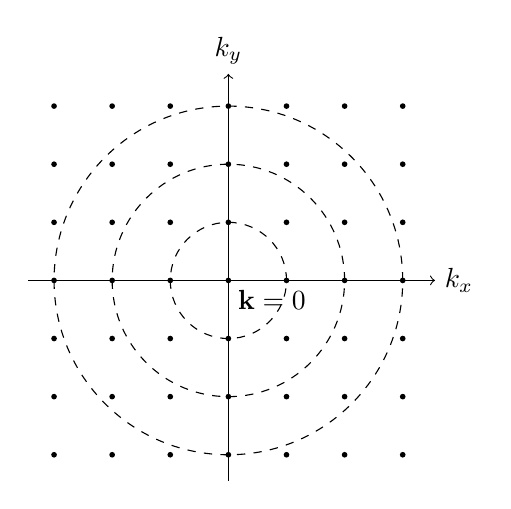
\begin{tikzpicture}[scale=0.82]
\draw[->] (-3.1,0) -- (3.2,0) node[right] {$k_x$};
\draw[->] (0,-3.1) -- (0,3.2) node[above] {$k_y$};
\draw[dashed] (0,0) circle (0.9);
\draw[dashed] (0,0) circle (1.8);
\draw[dashed] (0,0) circle (2.7);
\foreach \x in {-3,-2,-1,0,1,2,3}{
  \foreach \y in {-3,-2,-1,0,1,2,3}{
    \fill (0.9*\x,0.9*\y) circle (1.25pt);
  }
}
\node[below right] at (0,0) {$\mathbf{k}=0$};
\end{tikzpicture}
\caption{Дискретные импульсные состояния и оболочки постоянной энергии для частиц в конечном ящике с периодическими граничными условиями.}
\end{figure}

Для нерелятивистской частицы,
\begin{equation}
E_{\mathbf{k}}=\frac{\mathbf{k}^2}{2m},
\end{equation}
поэтому состоянием с наименьшей энергией является \(\mathbf{k}=0\). Поместим в ящик \(N\) тождественных бозонов и найдём основное состояние многочастичной системы. Первый бозон попадает в состояние с нулевым импульсом. Второй может попасть в то же состояние; так же могут поступить третий и каждый следующий бозон. Таким образом, все \(N\) бозонов занимают \(\mathbf{k}=0\).

Это бозонный конденсат: большое число тождественных частиц, занимающих одно и то же одночастичное состояние, здесь — состояние с наименьшей энергией. Волновая функция с нулевым импульсом постоянна в пространстве и простирается по всему ящику. Она не локализует какой-либо бозон в определённом месте; соответственно, положение каждого бозона неопределённо. Когда число частиц в этом состоянии становится большим, общая волновая функция создаёт макроскопическую амплитуду поля, и поле всё больше ведёт себя как классическое.

Основное состояние фермионов совершенно иное. Пока пренебрежём спином, так что каждой точке импульсного пространства соответствует одно доступное состояние. Первый фермион попадает в \(\mathbf{k}=0\), но второй тождественный фермион не может занять это же состояние. Следующие частицы должны занять следующую по энергии оболочку. На двумерном рисунке имеются четыре ближайшие ненулевые точки решётки с одинаковой энергией; в трёх измерениях их шесть. После заполнения этих состояний последующие частицы должны занимать следующие оболочки.

Поскольку энергия пропорциональна квадрату расстояния от начала координат в импульсном пространстве, минимизация полной энергии означает, что занятые точки нужно размещать как можно ближе к \(\mathbf{k}=0\), насколько это позволяет принцип исключения. При большом числе фермионов занятая область приближённо имеет форму сферы. Её граница — это поверхность Ферми, её внутренность — море Ферми, а вся заполненная область — сфера Ферми. При конечном объёме граница слегка зубчатая, потому что доступные точки образуют решётку, но для большой системы эта деталь становится несущественной.

\begin{figure}
\centering
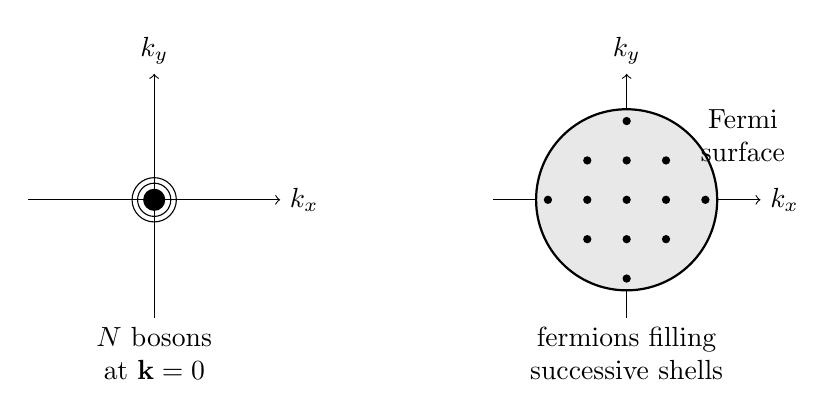
\begin{tikzpicture}[scale=1.0]
\begin{scope}[xshift=-3.0cm]
\draw[->] (-1.6,0) -- (1.6,0) node[right] {$k_x$};
\draw[->] (0,-1.5) -- (0,1.6) node[above] {$k_y$};
\fill (0,0) circle (4pt);
\draw (0,0) circle (6pt);
\draw (0,0) circle (8pt);
\node[align=center] at (0,-1.95) {$N$ bosons\\at $\mathbf{k}=0$};
\end{scope}
\begin{scope}[xshift=3.0cm]
\draw[->] (-1.7,0) -- (1.7,0) node[right] {$k_x$};
\draw[->] (0,-1.5) -- (0,1.6) node[above] {$k_y$};
\fill[gray!18] (0,0) circle (1.15);
\draw[thick] (0,0) circle (1.15);
\fill (0,0) circle (1.5pt);
\fill (0.5,0) circle (1.5pt);
\fill (-0.5,0) circle (1.5pt);
\fill (0,0.5) circle (1.5pt);
\fill (0,-0.5) circle (1.5pt);
\fill (0.5,0.5) circle (1.5pt);
\fill (0.5,-0.5) circle (1.5pt);
\fill (-0.5,0.5) circle (1.5pt);
\fill (-0.5,-0.5) circle (1.5pt);
\fill (1,0) circle (1.5pt);
\fill (-1,0) circle (1.5pt);
\fill (0,1) circle (1.5pt);
\fill (0,-1) circle (1.5pt);
\node[right,align=center] at (0.82,0.82) {Fermi\\surface};
\node[align=center] at (0,-1.95) {fermions filling\\successive shells};
\end{scope}
\end{tikzpicture}
\caption{Бозоны конденсируются в состояние с нулевым импульсом, тогда как фермионы заполняют импульсные состояния от центра наружу вплоть до поверхности Ферми.}
\end{figure}

Фермионное основное состояние имеет гораздо большую энергию, чем соответствующее бозонное основное состояние. Все бозоны могут оставаться при нулевом импульсе, но большинство фермионов вынуждено находиться в состояниях с ненулевым импульсом. По мере добавления новых фермионов максимальный занятый импульс растёт. Кроме того, оболочка при большом импульсе содержит больше точек решётки, чем оболочка вблизи начала координат. Поэтому большая сфера Ферми содержит много частиц со значительным импульсом и лишь небольшое число частиц в состояниях с наименьшим импульсом.

Контраст сохраняется и в возбуждённых состояниях. Для бозонов первое возбуждение получается переводом любого одного бозона из конденсата в первое возбуждённое одночастичное состояние:
\begin{equation}
(N,0,0,\ldots)\longrightarrow (N-1,1,0,\ldots).
\end{equation}
Не имеет значения, какой именно бозон переводится: частицы тождественны. Более высокие возбуждения можно получить несколькими способами. В зависимости от расстояния между уровнями можно поместить один бозон на более высокий уровень или два бозона на первый возбуждённый уровень. Возбудить бозонную систему — значит перевести частицы из конденсата в состояния с более высокой энергией.

Для фермионов никакую частицу нельзя перенести в другую точку внутри заполненной сферы Ферми, потому что каждая такая точка уже занята. Взять фермион из глубины моря и поместить его над поверхностью можно, но это требует большой энергии. Наименее затратное возбуждение берёт фермион из области сразу под поверхностью Ферми и переводит его в незанятое состояние сразу над ней. Переведённый электрон имеет лишь небольшую энергию над поверхностью, а оставленное им вакантное состояние лежит лишь немного ниже неё по энергии.

\begin{figure}
\centering
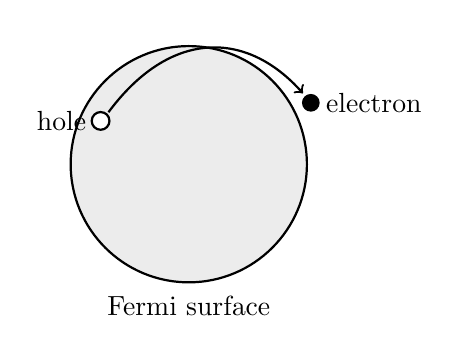
\begin{tikzpicture}[scale=1.0]
\fill[gray!15] (0,0) circle (1.5);
\draw[thick] (0,0) circle (1.5);
\draw[fill=white,thick] (-1.12,0.55) circle (3.2pt);
\fill (1.55,0.78) circle (3.2pt);
\draw[->,thick] (-1.02,0.66) .. controls (-0.25,1.7) and (0.72,1.72) .. (1.45,0.9);
\node[left] at (-1.18,0.55) {hole};
\node[right] at (1.62,0.78) {electron};
\node[below] at (0,-1.55) {Fermi surface};
\end{tikzpicture}
\caption{Низкоэнергетическое фермионное возбуждение переводит электрон через поверхность Ферми и оставляет дырку.}
\end{figure}

\section{Дырки и низкоэнергетические возбуждения}

Чтобы сделать заряд дырки наглядным, представим, что ящик содержит положительный заряд, равномерно размазанный по всему его объёму. В веществе этот положительный заряд в конечном счёте создаётся протонами в ядрах, но равномерное распределение сохраняет простоту модели. Добавим достаточно электронов, чтобы нейтрализовать фон. В основном состоянии эти электроны заполняют сферу Ферми.

Перевод одного электрона из-под поверхности Ферми над неё не изменяет полного заряда ящика. При этом возникает отрицательно заряженный электрон над поверхностью, а под ней остаётся недостающий отрицательный заряд. Поэтому отсутствующий электрон можно рассматривать как положительно заряженное возбуждение: дырку.

\begin{classroomqa}
\lecturetimestamp{01:31:38}
\audiencequestion{Имеет ли дырка ниже поверхности Ферми отрицательную энергию?}
\lecturerresponse{Нет. Дырка — это возбуждение над многочастичным основным состоянием, поэтому её энергия возбуждения положительна. Удаление занятого электрона из состояния ниже поверхности Ферми требует положительной затраты энергии, если энергии отсчитываются от этой поверхности.}
\end{classroomqa}

Пусть удалённый электрон имеет энергию \(\varepsilon<\varepsilon_F\), а переведённый электрон — энергию \(\varepsilon'>\varepsilon_F\). Сообщённую энергию можно разложить на две положительные разности энергий относительно поверхности Ферми.\footnote{Эти два интервала сформулированы по отдельности; приведённое здесь компактное равенство — алгебраически эквивалентная реконструкция.}
\begin{equation}
\Delta E
=\varepsilon'-\varepsilon
=(\varepsilon'-\varepsilon_F)+(\varepsilon_F-\varepsilon).
\end{equation}
Первый вклад естественно приписать электрону над поверхностью Ферми, а второй — дырке под ней:
\begin{equation}
E_{\mathrm{electron}}=\varepsilon'-\varepsilon_F>0,
\qquad
E_{\mathrm{hole}}=\varepsilon_F-\varepsilon>0.
\end{equation}
Электрон несёт отрицательный заряд, а дырка — положительный.

Электрон над поверхностью Ферми позже может перейти в доступную дырку. Тогда его энергия уменьшается, поэтому высвободившуюся энергию должно унести излучение. Это событие можно описать как переход электрона в незанятое состояние с меньшей энергией с испусканием одного или нескольких фотонов. Эквивалентно можно сказать, что электрон и дырка аннигилируют в излучение. Дырка не является дополнительной фундаментальной составляющей ящика; это отсутствие электрона в заполненном многоэлектронном состоянии. Тем не менее её энергия и заряд делают полезным рассматривать её как частицеподобное возбуждение.

\begin{classroomqa}
\lecturetimestamp{01:36:52}
\audiencequestion{Означает ли перевод электрона его перемещение из одной точки решётки в другую в импульсном пространстве?}
\lecturerresponse{Это означает перевод электрона с одного энергетического уровня на другой. Для свободных частиц в ящике импульсная решётка служит метками этих уровней, но сама идея не зависит от решётки в импульсном пространстве. В атоме положительный заряд сосредоточен в ядре. Электроны заполняют самые низкие доступные атомные уровни, и фотон может перевести один электрон на возбуждённый уровень, оставив вакансию на уровне, с которого тот был переведён. Эта вакансия — атомный аналог дырки.}
\end{classroomqa}

В ящике поглощение фотона аналогичным образом превращает энергию фотона в электрон над поверхностью Ферми и дырку под ней. В атоме та же терминология описывает возбуждённый электрон вместе с вакансией, оставшейся среди занятых нижних уровней.

\begin{classroomqa}
\lecturetimestamp{01:39:16}
\audiencequestion{Может ли низкоэнергетический фотон быть поглощён электроном где угодно в сфере Ферми?}
\lecturerresponse{Нет. Если электрон находится глубоко в море Ферми, все близлежащие состояния уже заняты, и низкоэнергетический фотон не может поднять его настолько, чтобы перевести в незанятое состояние над поверхностью. Только у электронов, достаточно близких к поверхности Ферми, имеются доступные пустые состояния в пределах энергетического диапазона фотона. Фотон с достаточно большой энергией может возбудить электрон из глубины моря.}
\end{classroomqa}

Поэтому сечение поглощения при низких энергиях определяется поверхностью моря Ферми, а не всем его объёмом. Электроны глубоко в море не могут совершать малые переходы; электроны чуть ниже поверхности можно перевести чуть выше неё.

\begin{classroomqa}
\lecturetimestamp{01:40:42}
\audiencequestion{Что мешает электронам взаимодействовать непосредственно друг с другом без падающего фотона?}
\lecturerresponse{Ничто. В этой простой модели электрон--электронными взаимодействиями пренебрегают, потому что их учёт делает картину моря Ферми более сложной. В этом первом приближении к металлу их эффективное влияние считается достаточно слабым, так что им обычно можно пренебречь.}
\end{classroomqa}

\begin{classroomqa}
\lecturetimestamp{01:41:10}
\audiencequestion{Что происходит, если один фотон несёт достаточно энергии, чтобы возбудить несколько электронов?}
\lecturerresponse{В принципе возможен любой процесс, согласующийся с законами сохранения. Фотон может создать не одну пару электрон--дырка: возбуждение двух электронов также оставляет две дырки. Такой процесс создаёт больше возбуждений и, как правило, менее вероятен, чем вариант, при котором эта энергия идёт на гораздо более сильное возбуждение одного электрона.}
\end{classroomqa}

\begin{classroomqa}
\lecturetimestamp{01:42:06}
\audiencequestion{Могут ли два фотона поглотиться вместе, когда ни один из них по отдельности не может вызвать это возбуждение?}
\lecturerresponse{Да. Поглощение носит вероятностный характер, и двухфотонный процесс может произойти, когда суммарная энергия фотонов достигает доступного возбуждения, хотя энергия каждого из них по отдельности ниже требуемой. Если имеющееся излучение несёт слишком мало энергии, чтобы достичь какого-либо разрешённого возбуждения, оно в основном проходит через систему.}
\end{classroomqa}

\editorialnote{Краткое обсуждение в этом месте связывает поглощённое излучение с коллективным движением электронов, но его содержательные детали восстановить невозможно. Надёжно установлено лишь утверждение о том, что такой коллективный отклик сложнее, чем одночастичная картина частица--дырка.}

\begin{classroomqa}
\lecturetimestamp{01:43:49}
\audiencequestion{Почему взаимодействия электрон--электрон называют слабыми, если все электроны несут одинаковый отрицательный заряд?}
\lecturerresponse{Электроны погружены в компенсирующий положительный фон. Этот фон экранирует заряд электрона и уменьшает эффективное взаимодействие в этой упрощённой постановке. Само взаимодействие не исчезает; для его описания требуется экранирующий отклик среды.}
\end{classroomqa}

\begin{classroomqa}
\lecturetimestamp{01:44:41}
\audiencequestion{Будет ли экранирование обсуждаться позже?}
\lecturerresponse{Да. Экранирование важно, но его обсуждение отложено до того момента, когда взаимодействующую систему можно будет рассмотреть более полно.}
\end{classroomqa}

\section{Одномерное фермионное море и античастицы}

Конструкция с дырками указывает на античастицы. Ту же логическую структуру можно перенести от электронов в веществе к релятивистскому квантовому полю и его вакууму. В простейшем варианте используются одно пространственное измерение и безмассовое фермионное поле \(\psi(x,t)\). В единицах, где скорость света равна единице, две возможные линейные дисперсионные зависимости имеют вид
\begin{equation}
\omega=k,
\qquad\text{or}\qquad
\omega=-k.
\end{equation}
Явно будет рассмотрена первая ветвь.

\editorialnote{В завершающем обмене репликами чередуются несовместимые отождествления частиц. Надёжно установлена лишь следующая модель: некоторое безмассовое фермионное модельное поле в одном пространственном измерении, ограниченное одним направлением распространения.}

Для плоской волны
\begin{equation}
\psi(x,t)=e^{i(kx-\omega t)},
\end{equation}
производные равны
\begin{equation}
\frac{\partial\psi}{\partial t}=-i\omega\psi,
\qquad
\frac{\partial\psi}{\partial x}=ik\psi.
\end{equation}
Следовательно, условие \(\omega=k\) эквивалентно полевому уравнению первого порядка
\begin{equation}
\frac{\partial\psi}{\partial t}
=-\frac{\partial\psi}{\partial x}.
\end{equation}

\begin{figure}
\centering
\includegraphics[width=0.72\textwidth]{lecture_05_figure_05.png}
\caption{Начало вывода полевого уравнения первого порядка, плоские волны которого удовлетворяют \(\omega=k\).}
\lectureframe{01:47:22}
\end{figure}

Любой профиль вида \(f(x-t)\) удовлетворяет этому уравнению и движется вправо. Изменение знака даёт
\begin{equation}
\frac{\partial\psi}{\partial t}
=+\frac{\partial\psi}{\partial x},
\end{equation}
для которого профили \(f(x+t)\) движутся влево. Каждое из этих уравнений первого порядка выделяет только одно направление движения. Будем считать поле фермионным и, в рамках рассуждения о дырках, предположим, что его частицы несут электрический заряд.

Ветвь \(\omega=k\) сразу порождает трудность. Волновое число \(k\) может быть отрицательным, и поэтому отрицательным может быть и \(\omega\). Поскольку \(\omega\) в этих единицах является энергией, линейный спектр содержит состояния как с положительной, так и с отрицательной энергией:
\begin{equation}
E=\omega=k.
\end{equation}

\begin{figure}
\centering
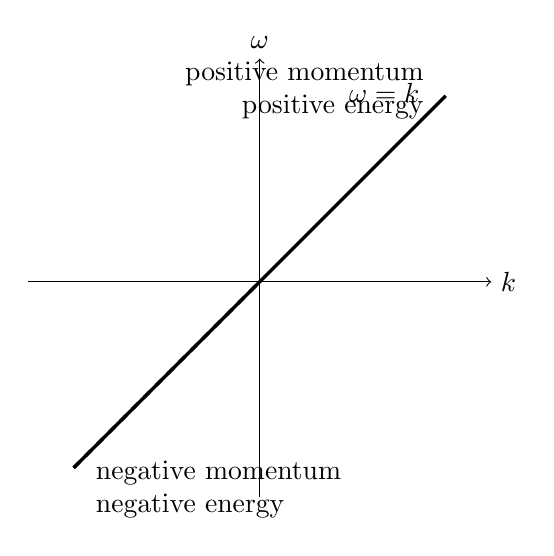
\begin{tikzpicture}[scale=1.05]
\draw[->] (-2.8,0) -- (2.8,0) node[right] {$k$};
\draw[->] (0,-2.6) -- (0,2.7) node[above] {$\omega$};
\draw[very thick] (-2.25,-2.25) -- (2.25,2.25);
\draw[very thick,dashed] (-2.25,-2.25) -- (0,0);
\node[above left] at (2.05,2.05) {$\omega=k$};
\node[below right,align=left] at (-2.1,-2.05) {negative momentum\\negative energy};
\node[above left,align=right] at (2.1,1.85) {positive momentum\\positive energy};
\end{tikzpicture}
\caption{Одноветвевой спектр \(\omega=k\); его половина при \(k<0\) соответствует отрицательной энергии.}
\end{figure}

Обычный пустой вакуум не может быть основным состоянием такой теории. Фермион с положительной энергией мог бы излучить фотон и перейти в состояние с меньшей энергией. Ничто не заставило бы его остановиться на нуле: он мог бы продолжить переходить в состояния с отрицательной энергией, испускать всё больше излучения и падать без ограничения. Энергия, потерянная фермионом, появлялась бы в поле излучения. Поэтому спектр, не ограниченный снизу, не даёт устойчивого обычного вакуума.

Фермионный запрет даёт другую исходную точку. Заполним каждое одночастичное состояние с отрицательной энергией, вплоть до нулевой энергии, одним фермионом. Ни один дополнительный фермион не может упасть в эти состояния, потому что каждое из них уже занято. Добавить ещё один фермион с отрицательной энергией невозможно, тогда как добавление фермиона с положительной энергией повышает энергию. Поэтому полностью заполненное море отрицательной энергии можно принять за многочастичное основное состояние и назвать вакуумом.

\begin{figure}
\centering
\resizebox{\linewidth}{!}{%
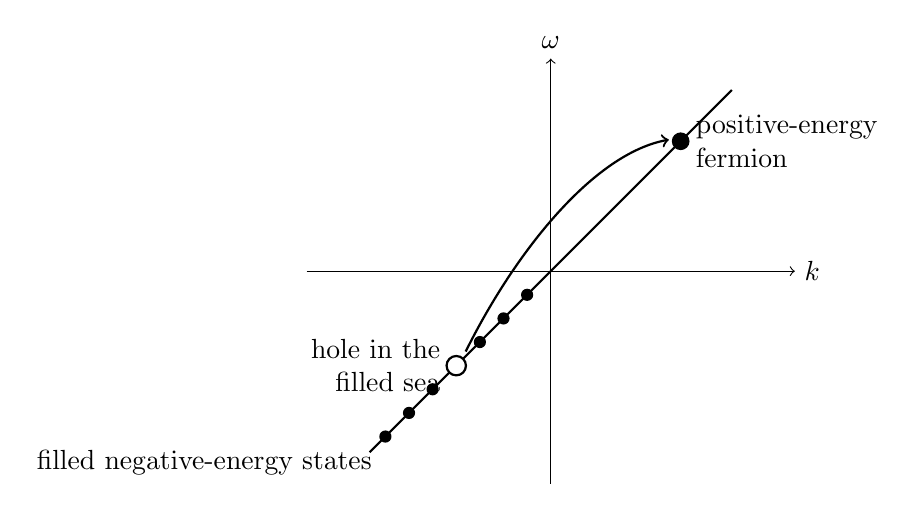
\begin{tikzpicture}[scale=1.0]
\draw[->] (-3.1,0) -- (3.1,0) node[right] {$k$};
\draw[->] (0,-2.7) -- (0,2.7) node[above] {$\omega$};
\draw[thick] (-2.3,-2.3) -- (2.3,2.3);
\foreach \p in {-2.1,-1.8,-1.5,-1.2,-0.9,-0.6,-0.3}{
  \fill (\p,\p) circle (2.2pt);
}
\draw[fill=white,thick] (-1.2,-1.2) circle (3.5pt);
\fill (1.65,1.65) circle (3.2pt);
\draw[->,thick] (-1.08,-1.02) .. controls (-0.45,0.25) and (0.55,1.5) .. (1.5,1.67);
\node[left,align=right] at (-1.28,-1.2) {hole in the\\filled sea};
\node[right,align=left] at (1.72,1.65) {positive-energy\\fermion};
\node[below left] at (-2.15,-2.15) {filled negative-energy states};
\end{tikzpicture}%
}
\caption{Заполненное море отрицательной энергии и возбуждение, образованное переводом одного фермиона на положительную энергию.}
\end{figure}

Простейшее возбуждение состоит в том, что один фермион удаляется из моря отрицательной энергии и помещается в состояние с положительной энергией. Переведённый фермион является обычной частицей с положительной энергией. Освободившееся в море место — это второе возбуждение, дырка. Если удалённый фермион имеет отрицательный заряд, дырка имеет положительный заряд.

В этом одноветвевом примере дырка также имеет положительный импульс. Если отсутствующий фермион занимал состояние с импульсом \(k_-<0\), то его удаление изменяет полный импульс на
\begin{equation}
p_{\mathrm{hole}}=-k_->0.
\end{equation}
Это дефицит отрицательного импульса. Таким образом, возбуждение состоит из отрицательно заряженного фермиона с положительной энергией и положительно заряженной дырки с положительной энергией. Оба возбуждения несут положительный импульс и на ветви \(\omega=k\) движутся вправо.

В полной электронной теории положительно заряженная дырка — это позитрон. Первоначально Dirac рассматривал возможность отождествить дырку с протоном. Эта конструкция требует, чтобы частица и её античастица имели одинаковую массу. Дырка — отдельная частица с массой электрона и противоположным электрическим зарядом. Это и есть основная интерпретация частица--античастица, к которой привёл спектр отрицательных энергий.

Тот же выход нельзя применить к бозонам. Бозонное состояние допускает сколь угодно много частиц, так что невозможно один раз заполнить уровень отрицательной энергии и тем самым заблокировать его дальнейшее заселение. На этот уровень всегда можно было бы добавлять ещё бозоны, снова и снова понижая энергию:
\begin{equation}
\begin{aligned}
\text{fermionic mode: }&n=0\ \text{or}\ 1,\\
\text{bosonic mode: }&n=0,1,2,\ldots .
\end{aligned}
\end{equation}
Предлагаемая бозонная система всё равно не имела бы основного состояния. В этой элементарной конструкции устойчивость заполненного моря зависит именно от фермионного запрета.

Это одномерное уравнение — лишь модельная версия уравнения Dirac. Его поле безмассово, движется со скоростью света и распространяется только в одном направлении. Более полное уравнение Dirac должно учитывать недостающие направления движения и остальную структуру релятивистской частицы. Обсуждение этого более полного уравнения, вместе с рассмотрением античастиц для бозонных полей, откладывается.
